\newpage
\chapter{Proposed Method}
\section{Deep Learned Features for Action Recognition in First-Person Video}

asd 
\begin{figure}[htttp]
\centering
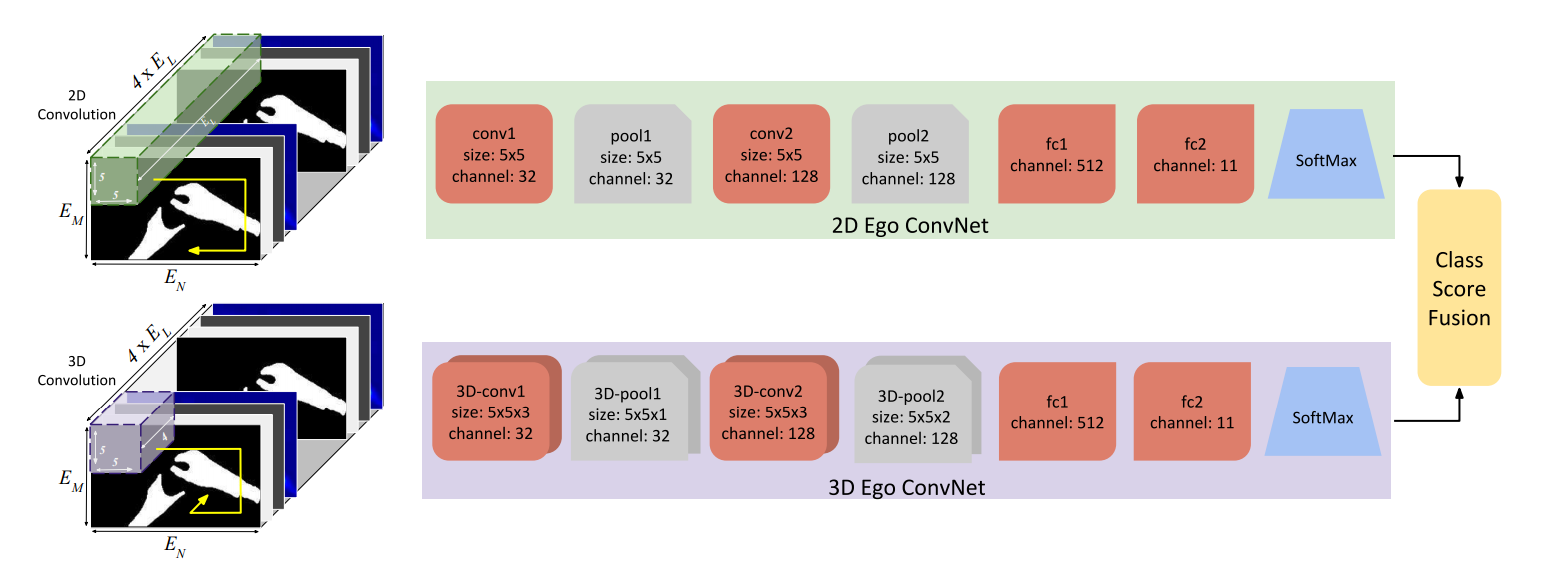
\includegraphics[width=1\textwidth]{figures/framework2}
\caption{Overview of the proposed action recognition scheme for the first-person video.
} 
\label{fig:framework}
%\vspace{-4mm}
\end{figure}

\section{Temporal Aggregation Using Hilbert-Huang Transform }

In this section, we introduce the proposed  HHT-based temporal
aggregation  method for first-person videos. The new method begins
with feature extraction using CNN \cite{wang2015action} and then
invokes HHT on the features by first decomposing the features with
EMD and conducting time-frequency analysis with Hilbert transform
for each IMF decomposed features. Finally, we analyze the
statistical properties of some desirable features to construct our
feature representation. For easy reference, the overall procedures
of the proposed method are as illustrated in Fig.
\ref{fig:framework}.

\subsection{Trajectory-pooled Deep-convolutional Descriptors}
In this section, we briefly review the TDD feature extraction
\cite{wang2015action}. % We  first use the trajectory-pooled
%deep-convolutional descriptors.
The deep-learned based features takes advantage of the image
appearance and motion information as descriptors.
%. This deep-learned
It first uses the ConvNets architecture and is trained on large
datasets in order to extract multi-scale convolutional maps. Then,
TDD employs the improved trajectories to aggregate an efficient
feature representation by sampling and pooling. We also apply both
spatio-temporal and channel normalization to the TDD features to
boost the performance. Finally, we combine those features to
obtain a TDD feature vector.

\begin{figure}[!t]
\centering
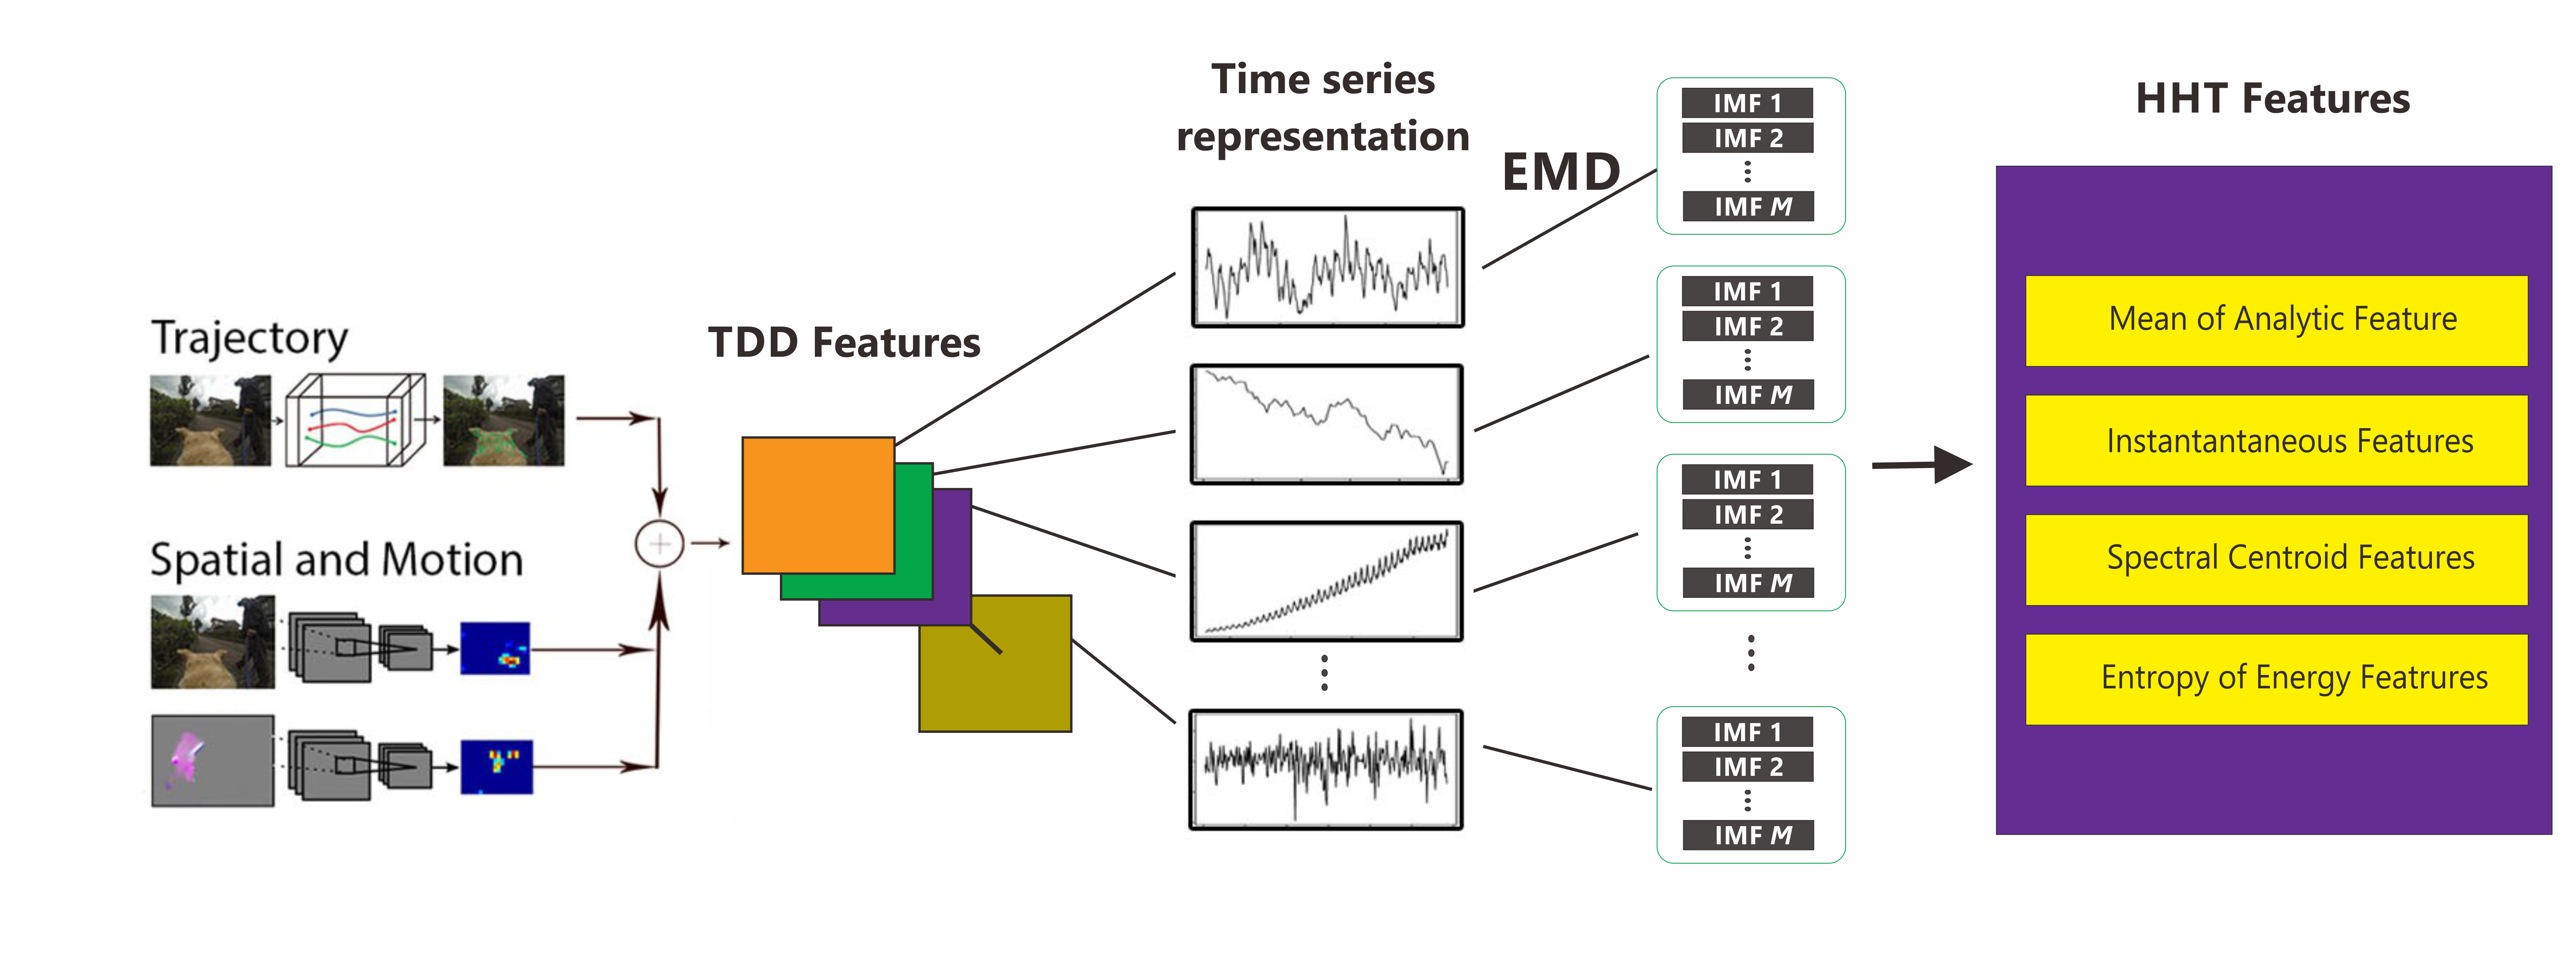
\includegraphics[width=1\textwidth]{figures/framework}
\caption{Overview of the proposed action recognition scheme for the first-person video.
} 
\label{fig:framework}
%\vspace{-4mm}
\end{figure}

\subsection{Empirical Mode Decomposition}

After determining the TDD descriptors in feature extraction,
this subsection describes EMD, a way to decompose signals into a
number of IMFs. Given a feature descriptor, which is in general
non-stationary, with dimension  $k \times l$, where $k$ and $l$ are
the numbers of the spatio-temporal features and  feature channel,
respectively, we apply EMD to the descriptor in each feature channel
to obtain a set of IMFs by the following steps, where for simplicity
the feature is denoted as $x(n)$.
\begin{enumerate}
    \item Identify both maxima and minima (extremes) of  $x(n)$.
    \item Interpolate between minima and maxima to generate the envelopes  $e_{l}(n)$ and $e_{m}(n)$.
    \item Calculate the local mean by  $a(n)=(e_{m}(n)+e_{n}(n))/2$.
    \item Extract the detail  $h_{1}(n) = x(n) - a(n)$.
    \item Decide whether $h_{1}(n)$ is IMF or not. If the number of extremes and zero crossing of  $h_{1}(n)$ are the same or differ by at most one and at any point the average value of the envelope defined by both local maxima and minima are zero, then  $h_{1}(n)$  is regarded as IMF; otherwise, it is not.
    \item Repeat steps 1 to 5 until we get all of IMFs.
\end{enumerate}

Finally, $x(n)$ can be represented as
\begin{equation}
      x(n) = \sum_{m=1}^{M} c_{m}(n) + r_{M}(n)
\end{equation}
where $M$ denotes the number of IMFs, $c_{m}(n)$ is the $m$th IMF of
the feature  $x(n)$ and $r_{M}(n)$ stands for the residue.

\subsection{Hilbert Transform Analysis}
Based on the IMFs determined above, this subsection
describes the Hilbert transform analysis  to extract the desired
features. For this, we conduct the Hilbert transform with
respect to IMFs and obtain
analytic signals %which will be used as our first feature.
%%Denote IMF as $c_{m}(t)$,
%we  determine our analytic signals by the Hilbert transform
%given by




\begin{equation}
{\cal H}[c_{m}(n)] = \frac{1}{\pi}\sum_{n' = 1 }^{K
}\frac{c_{m}(n')}{n-n'}
\end{equation}
where $K$ is the length of $c_{m}(n)$. The associated analytic
signal can then be expressed as


\begin{equation}
    z_{m}(n) = c_{m}(n) + jH[c_{m}(n)] = a_{m}(n)e^{j\phi_{m}(n)}
\end{equation}

%Based on {\blue $z_{m}(n)$},
Next, we consider four features associated with the
%statistical
characteristics of $z_{m}(n)$, {\it i.e.} mean,
instantaneous frequency, spectral centroid \cite{riaz2016emd}, and
entropy of energy \cite{tolwinski2007hilbert}. The  mean feature of
$z_{m}(n)$  is given by
\begin{equation}
    \mu_{m}(n) = \frac{1}{K}\sum_{n=1}^{K} z_{m}(n)
\end{equation}


The instantaneous frequency feature %of each IMF
is given by
\begin{equation}
f_{m}(n) = \frac{1}{4\pi}(\phi_{m}(n+1)-\phi_{m}(n-1))
\end{equation}

%Apart from instantaneous frequency, we also  take the spectral centroid information \cite{riaz2016emd} as our third feature {\blue by
The spectral centroid feature,  $C_{s}^{m} $, is given by
\begin{equation}
    C_{s}^{m} = \frac{\sum_{f_{m}}2 \pi f_{m}P(f_{m})}{\sum_{f_{m}}P(f_{m})}
\end{equation}
where $P(w)$ is power spectral density of  $z_{m}(n)$
\cite{riaz2016emd}.

The log of entropy feature is given by
\begin{equation}
    H_{m} = - \sum_{i=1}^{N}p_{i} \ \textup{log} \ p_{i}
\end{equation}
where $p_{i}$ is the probability of energy level $E_{i}
=log(\sum_{n=1}^{K}|z_{m}(n)|^{2})$ appears.


Finally, we can use these four features individually or
combine them together into a single feature vector as our final
feature representation.

